\chapter{Tests}
\label{ch:tests}

Se han creado 5 sujetos de prueba con diferentes características para la experimentación. Dado que los algoritmos son estocásticos, se seleccionaron 31 semillas distintas para garantizar la reproducibilidad de las ejecuciones. Por lo tanto, se han realizado 155 tests por cada configuración. En el anexo \ref{ch:entorno-sujetos} se encuentran detallados todos los sujetos de prueba, los \textit{seeds} y el entorno usado para la ejecución de las pruebas.

Para trabajar con los sujetos, y poder añadir más en el futuro sin tocar el código fuente, se ha creado una tabla \textit{''sujetos''} en la base de datos, cuyos campos son: \textit{''id''}, \textit{''peso''}, \textit{''altura''}, \textit{''edad''}, \textit{''sexo''} y \textit{''actividad''}. Estos dos últimos son de tipo \textit{''enum''} para que solo puedan tener valores predefinidos, explicados en el apartado \ref{ch:calculo-calorías}. Para visualizar las calorías correspondientes a cada sujeto se ha establecido una vista \textit{''sujeto\_calorias''}, que realiza los cálculos necesarios a partir de los datos de la tabla \textit{''sujetos''}, lo que permite visualizar fácilmente el objetivo calórico de cada individuo de prueba.

Se ha diseñado un modelo de relaciones \textit{N:N}, donde los sujetos tienen una relación con los grupos de alimentos. Debido a que cada sujeto puede gustarle o ser alérgico a varios grupos de alimentos, se han creado tres tablas intermedias: \textit{''sujeto\_gustos''}, \textit{''sujeto\_disgustos''} y \textit{''sujeto\_alergias''}. Las 3 tablas tienen un campo que representa al sujeto y otro al grupo de comida.

En la figura \ref{fig:sujetos-prueba} se muestra el resultado de la consulta que recupera toda la información asociada a los sujetos de prueba creados.
\begin{figure}[H]
    \centering
    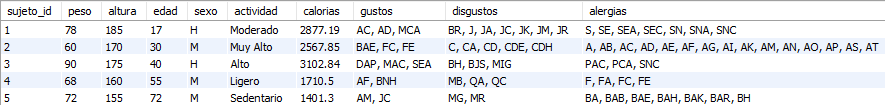
\includegraphics[width=1\textwidth]{figures/sujetos_prueba.png}
    \caption{Sujetos de prueba.}
    \label{fig:sujetos-prueba}
\end{figure}
\newpage
El primer paso fue realizar un análisis de sensibilidad. Se probaron diferentes valores para cada hiperparámetro (tipos de operadores, probabilidad, tamaño de la población, ...) y se han comparado para poder encontrar la mejor configuración posible.

Para comparar conjuntos de resultados se han usado dos métodos. El primero, \textit{success rate}, mide la viabilidad de cada configuración, evaluando el número de soluciones factibles que propone. La mejor configuración es la que mayor tasa de éxito tiene.

El otro método para poder hacer comparaciones entre las configuraciones de un problema multiobjetivo es calculando el \textit{hipervolumen}, que evalúa la calidad de un conjunto de soluciones. Mide el volumen de la región del espacio que está dominada por las soluciones del conjunto y una referencia externa. Cuanto mayor sea, mejor será la calidad de las soluciones y la diversidad~\cite{pymoo2024hypervolume}. Solo se han calculado los hipervolumenes de las soluciones factibles, eliminando las que no cumplen las restricciones.

Para comparar hipervolumenes se hace uso de un test de significatividad estadística. Se trata de una prueba estadística que propone una hipótesis nula (\(H_0\) ), es decir, que ambos conjuntos provienen de la misma distribución, ya que no existe una diferencia significativa entre las muestras. El test devuelve un \textit{''p\_value''} que señala qué tan probable es \(H_0\). Si el valor \textit{p} es inferior a un umbral ($\alpha$), que suele ser 0.05, se puede rechazar \(H_0\). Esto quiere decir que hay una probabilidad menor del 5\% de que dos muestras vengan de la misma distribución.

Rechazar \(H_0\) proporciona evidencia en contra de la hipótesis y que, efectivamente, existe una diferencia significativa entre los conjuntos. Sin embargo, no rechazar \(H_0\) deja en un estado de incertidumbre y solo indica que no se tiene suficiente evidencia para descartarla.

Según el número de conjuntos a comparar se pueden usar diversos tests no paramétricos. En este caso, este trabajo se ha centrado en dos.

Para la comparación de dos conjuntos de resultados se usa el \textit{test de rangos con signos de Wilcoxon}. El proceso calcula las diferencias entre pares (en total 31), ordena los resultados absolutos y les asigna un rango. Después suma los rangos de las diferencias positivas y negativas por separado. La prueba se queda con el valor menor. Si el valor es menor que un valor crítico, obtenido de una tabla de Wilcoxon, se rechaza la hipótesis nula.~\cite{scipy2024wilcoxon}

Para la comparación de \textit{n} conjuntos se usa el \textit{test de rangos alineados de Friedman}. Dentro de cada conjunto se ordenan los valores de menor a mayor, dándoles a cada uno un rango de manera ascendente. Se calcula la media de todos los valores con el mismo rango y este valor se resta a cada uno de los números que presenten ese rango. Se suman los rangos que sean iguales entre todos los conjuntos. Es decir, el rango 1 del primer conjunto se suma con el rango 1 del segundo conjunto, y así sucesivamente con todos los rangos. Estas sumas son introducidas en la fórmula de Friedman. El resultado de esta fórmula se compara con un valor crítico de la distribución chi-cuadrado. Al igual que en la de Wilcoxon, si el resultado es menor que el valor crítico, se rechaza \(H_0\).~\cite{stac2024friedman}

El problema de este método es que no determina qué conjunto de resultados es mejor. Si se comparase cada par de conjuntos por separado la probabilidad de error por cada comparativa se iría acumulando, haciendo las siguientes comparativas inviables. Por ello se propone la variación del test de \textit{rangos alineados de Friedman} con la corrección \textit{post-hoc} de \textit{Shaffer}. Permite realizar comparaciones más precisas entre cada par de conjuntos.~\cite{stac2024shaffer}

Si se rechaza \(H_0\), se comparan las medias y las desvianzas típicas de los hipervolúmenes para saber qué conjunto de resultados es mejor.

Tras haber analizado individualmente cada configuración de hiperparámetros del algoritmo, ya se puede hacer la comparación entre las variaciones del algoritmo propuestas.

\section{Manejo de restricciones}
\label{ch:manejo-restricciones-experimentacion}

Todas las tablas de resultados y comparación de hiperparámetros, expuestas en el apéndice \ref{ch:tablas-resultados}, van a seguir la misma estructura, la cual se muestra en la tabla \ref{table:resultados-penalizacion-estatica-mutacion}. Cada fila muestra los resultados para un sujeto en una configuración de hiperparámetros. En este proyecto se ha comparado la probabilidad de mutación y el tipo y probabilidad de cruce. Por cada sujeto se muestra el tiempo en ejecutar un test, siendo este resultado una media de los 31 tests antes mencionados. Las dos siguientes columnas muestran el número de soluciones que se han obtenido de media entre todas las ejecuciones y el número medio de esas soluciones que son factibles, respectivamente. La columna final muestra el \textit{success rate}, dividiendo el número de soluciones factibles entre el número total de soluciones.

Las tablas del método separatista presentan modificaciones, ya que todas las soluciones que muestra este procedimiento son factibles. Por lo tanto, en vez de mostrar el número de soluciones factibles, se muestra el número de ejecuciones que han obtenido soluciones factibles. El \textit{success rate} se calcula dividiendo este nuevo número entre el total de ejecuciones realizadas para un sujeto en una configuración concreta, que es 31. En el anexo, la tabla \ref{table:resultados-metodo-separatista-mutacion-anexo} muestra la estructura a seguir en estos casos.

\begin{table}[H]
    \centering
    \scriptsize
    \begin{adjustbox}{max width=\textwidth}
    \begin{tabularx}{\textwidth}{|>{\centering\arraybackslash}X|>{\centering\arraybackslash}c|>{\centering\arraybackslash}X|>{\centering\arraybackslash}X|>{\centering\arraybackslash}X|>{\centering\arraybackslash}X|}   
    \specialrule{1.3pt}{0pt}{0pt}
    \textbf{Tipo de Mutación} & \textbf{Sujeto} & \textbf{Tiempo Medio de Ejecución (s)} & \textbf{Media de Soluciones No Dominadas} & \textbf{Media de Soluciones Factibles} & \textbf{Success Rate} \\   
    \specialrule{1.3pt}{0pt}{0pt}
    \multirow{5}{*}{\textbf{Baja (1/77)}}
    & 1 & 6.11 & 26.16 & 25.94 & 99.14\% \\
    \cline{2-6}
    & 2 & 6.21 & 23.81 & 23.26 & 97.70\% \\
    \cline{2-6}
    & 3 & 6.08 & 28.13 & 28.00 & 99.54\% \\
    \cline{2-6}
    & 4 & 6.11 & 35.23 & 35.23 & 100.00\% \\
    \cline{2-6}
    & 5 & 6.25 & 63.84 & 63.84 & 100.00\% \\   
    \specialrule{1.3pt}{0pt}{0pt}
    \multirow{5}{*}{\textbf{Media (0.05)}}
    & 1 & 7.24 & 1.42 & 0.03 & 2.27\% \\
    \cline{2-6}
    & 2 & 7.51 & 1.32 & 0.26 & 19.51\% \\
    \cline{2-6}
    & 3 & 7.40 & 2.35 & 1.39 & 58.90\% \\
    \cline{2-6}
    & 4 & 7.40 & 3.81 & 3.23 & 84.75\% \\
    \cline{2-6}
    & 5 & 7.25 & 29.03 & 29.03 & 100.00\% \\   
    \specialrule{1.3pt}{0pt}{0pt}
    \multirow{5}{*}{\textbf{Alta (0.1)}}
    & 1 & 8.84 & 1.03 & 0.00 & 0.00\% \\
    \cline{2-6}
    & 2 & 8.97 & 1.03 & 0.00 & 0.00\% \\
    \cline{2-6}
    & 3 & 8.90 & 1.13 & 0.00 & 0.00\% \\
    \cline{2-6}
    & 4 & 8.91 & 1.00 & 0.00 & 0.00\% \\
    \cline{2-6}
    & 5 & 8.95 & 5.48 & 5.45 & 99.41\% \\  
    \specialrule{1.3pt}{0pt}{0pt}
    \end{tabularx}
    \end{adjustbox}
    \caption{Resultados en Penalización estática: probabilidad de mutación.}
    \label{table:resultados-penalizacion-estatica-mutacion}
\end{table}

El \textit{success rate} en las tablas de resultados sobre la probabilidad de mutación (\ref{table:resultados-penalizacion-estatica-mutacion} y \ref{table:resultados-metodo-separatista-mutacion-anexo}) indica que el algoritmo genera mejores soluciones cuanto menor es la probabilidad. La probabilidad baja favorece una convergencia más rápida y propone soluciones muchas veces similares entre sí, pero que cumplen con todas las restricciones.

Al contrario que la mutación, el cruce no altera en gran medida la viabilidad de las soluciones propuestas (tablas \ref{table:resultados-penalizacion-estatica-cruce-anexo} y \ref{table:resultados-metodo-separatista-cruce-anexo}). A partir de los resultados no se puede determinar cuál es la mejor configuración posible, por lo que es necesario la comparación de los hipervolúmenes. El test de Friedman, junto con la corrección post-hoc de Shaffer, muestra que el algoritmo con cruce de dos puntos y alta probabilidad es el más efectivo en todos los tipos de manejo de restricciones, lo que significa que la mejor opción es la que mayor recombinación de genes entre padres presenta, ayudando a mejorar la exploración del espacio de soluciones.
\newpage
La comparación de algoritmos se realiza entre el método separatista y la penalización estática, ya que los resultados que se obtienen con el método \textit{''ConstraintsAsObjective''} muestra resultados muy malos y soluciones no factibles en más del 95\% de los casos (tablas \ref{table:resultados-restriccion-objetivo-mutacion-anexo} y \ref{table:resultados-restriccion-objetivo-cruce-anexo}). La prueba de Wilcoxon obtiene un \textit{$p = 0.1037$}, por lo que no hay suficiente evidencia para demostrar que hay una diferencia significativa entre ambos conjuntos de resultados.

En la tabla \ref{table:comparacion-manejos-restricciones-grafico} se muestra de manera gráfica las conclusiones que se obtienen tras la comparación de los métodos. Como se ha explicado,  la calidad de las soluciones obtenidas con la penalización estática y el método separatista es prácticamente igual. En cuanto a la estabilidad, la penalización estática presenta un \textit{success rate} más cercano al 100\% en los sujetos 1, 2 y 3 respecto al método separatista. En cambio, en los tiempos de ejecución destaca el método separatista, que es, de media, 1 segundo más rápido que el otro procedimiento.

Por lo tanto, no es posible determinar cuál es el mejor método de manejo de restricciones con las pruebas realizadas con el algoritmo multiobjetivo NSGA-II. Ambos métodos van a ser usados en las pruebas de comparación de algoritmos para comprender la configuración de parámetros óptima para el proyecto.
\begin{center}
    {\color{red} \Large /// TODO: Apéndice de fitness (incluyendo NSGA3)///}
\end{center}

\begin{figure}[H]
    \centering
    \includegraphics[width=1\textwidth]{figures/graficas/nsga2_estatica/fitness_nsga2_penalizacion_estatica_calorías.png}
    \caption{Fitness NSGA-II. Objetivo calorías.}
    \label{fig:sujetos}
\end{figure}

\renewcommand{\arraystretch}{1.5}

\begin{table}[h!]
    \centering
    \begin{tabular}{|c|c|c|c|}
        \hline
        \textbf{Método de manejo de restricciones} & \textbf{Estabilidad} & \textbf{Calidad} & \textbf{Velocidad} \\
        \hline
        Penalización Estática & 
        \tikz{\node[draw=none, fill=green!30, rounded corners=2pt]{\scriptsize $\blacktriangle$};} & 
        \tikz{\node[draw=none, fill=yellow!30, rounded corners=2pt]{\scriptsize $\approx$};} & 
        \tikz{\node[draw=none, fill=yellow!30, rounded corners=2pt]{\scriptsize $\approx$};} \\
        \hline
        Método Separatista & 
        \tikz{\node[draw=none, fill=yellow!30, rounded corners=2pt]{\scriptsize $\approx$};} & 
        \tikz{\node[draw=none, fill=yellow!30, rounded corners=2pt]{\scriptsize $\approx$};} & 
        \tikz{\node[draw=none, fill=green!30, rounded corners=2pt]{\scriptsize $\blacktriangle$};} \\
        \hline
        Restricción como Objetivo & 
        \tikz{\node[draw=none, fill=red!60, rounded corners=2pt]{\scriptsize $\blacktriangledown$};} & 
        \tikz{\node[draw=none, fill=red!60, rounded corners=2pt]{\scriptsize $\blacktriangledown$};} & 
        \tikz{\node[draw=none, fill=red!60, rounded corners=2pt]{\scriptsize $\blacktriangledown$};} \\
        \hline
    \end{tabular}
    \caption{Comparación de métodos de manejo de restricciones.}
    \label{table:comparacion-manejos-restricciones-grafico}
    \vspace{0.5em}
    \raggedright
    Leyenda:
    \begin{itemize}
        \item \tikz{\node[draw=none, fill=green!30, rounded corners=2pt]{\scriptsize $\blacktriangle$};} Representa un desempeño superior.
        \item \tikz{\node[draw=none, fill=yellow!30, rounded corners=2pt]{\scriptsize $\approx$};} Representa un desempeño medio.
        \item \tikz{\node[draw=none, fill=red!60, rounded corners=2pt]{\scriptsize $\blacktriangledown$};} Representa un desempeño inferior.
    \end{itemize}
\end{table}

\renewcommand{\arraystretch}{1}
\newpage
\section{Algoritmos multi-objetivo}
\label{ch:algoritmos-multiobjetivo}

Por los resultados mostrados en la tabla \ref{table:resultados-spea2-anexo} no es posible saber el mejor método de manejo de restricciones con el algoritmo SPEA2, por lo que se realiza una prueba de Wilcoxon entre pares. El resultado arroja un \textit{$p = 0.87$}, por lo que no hay suficiente evidencia para demostrar que son diferentes.

Para MOEA/D se va a comparar diferente cantidad de vecinos, la probabilidad de selección de vecinos y el número de direcciones de referencia con dos métodos muy usados para generarlas, \textit{das-dennis} e \textit{incremental}, explicadas en el punto \ref{ch:moead}. Este algoritmo solo se va a probar con el método de penalización estática, ya que no permite restricciones explícitas.

Es interesante ver que todas las soluciones generadas por las distintas configuraciones de la tabla \ref{table:resultados-moead-nvecinos-anexo} son factibles, lo que puede demostrar que MOEA/D es un buen algoritmo para nuestro problema. Tras realizar el test estadístico, la mejor configuración es la que presenta un mayor número de vecinos, 30.

La probabilidad de selección entre vecinos tampoco supone un gran cambio en la factibilidad de las soluciones que propone el algoritmo (tabla \ref{table:resultados-moead-prob-vecinos-anexo}). Tras realizar el test para casos \textit{NxN}, no se encontró suficiente evidencia para rechazar \(H_0\). La media entre calidad, estabilidad y rapidez es más alta en la probabilidad más alta (0.9), por lo que es la que se usa.

Para establecer un número de direcciones con el método de generación \textit{das-dennis}, se compara el \textit{success rate} de la tabla \ref{table:resultados:moead-direcciones-dasdennis-anexo} y se realizan los tests no paramétricos. Aunque la que presenta un número más elevado de direcciones es la configuración con más calidad, se ha decidido seleccionar la configuración con 12 direcciones debido a los altos tiempos que necesita ''Alto (18)'' en cada ejecución, haciendo inviable su uso en un entorno real. Con los resultados obtenidos tras la generación de direcciones de referencia con \textit{incremental} ocurre lo mismo, el mayor número de direcciones arroja mejores resultados, pero los tiempos de ejecución elevados descartan esa configuración. Tras hacer el test de Wilcoxon entre ambas configuraciones, se concluye que \textit{incremental} presenta mejores soluciones que \textit{das-dennis}.

Con todas las configuraciones elegidas ya se puede realizar la comparación entre algoritmos. Los resultados muestran que, en cuanto a calidad de soluciones propuestas, el algoritmo de NSGA-II con el método separatista es el mejor, seguido por NSGA-II con penalización estática. En tercer y cuarto lugar se encuentra SPEA2 con penalización estática y con manejo separatista, respectivamente. Finalmente, el algoritmo MOEA/D tiene el peor rendimiento según los rankings obtenidos.

El MOEA/D presenta un success rate del 100\%. Los métodos de penalización estática, tanto de NSGA-II como de SPEA2, lo siguen de cerca, con más del 99\% de soluciones factibles propuestas. Los métodos separatistas empeoran un poco respecto al resto, aunque ambos siguen presentando más del 97\% de success rate.

En cuanto a los tiempos, todos los métodos de los algoritmos NSGA-II y SPEA2 no se llevan más de 1 segundo de diferencia, siendo el mejor el método separatista de NSGA-II con 5.64 segundos y el peor la penalización estática del mismo algoritmo con 6.61 segundos. El algoritmo con los peores tiempos es MOEA/D, donde la media sube a 8.76 segundos por ejecución.

\renewcommand{\arraystretch}{1.5}

\begin{table}[h!]
    \centering
    \begin{tabular}{|c|c|c|c|}
        \hline
        \textbf{Algoritmo} & \textbf{Estabilidad} & \textbf{Calidad} & \textbf{Velocidad} \\
        \hline
        NSGA-II (Penalización estática) & 
        \tikz{\node[draw=none, fill=yellow!30, rounded corners=2pt]{\scriptsize $\approx$};} & 
        \tikz{\node[draw=none, fill=green!30, rounded corners=2pt]{\scriptsize $\blacktriangle$};} & 
        \tikz{\node[draw=none, fill=yellow!30, rounded corners=2pt]{\scriptsize $\approx$};} \\
        \hline
        NSGA-II (Método separatista) & 
        \tikz{\node[draw=none, fill=red!60, rounded corners=2pt]{\scriptsize $\blacktriangledown$};} & 
        \tikz{\node[draw=none, fill=green!30, rounded corners=2pt]{\scriptsize $\blacktriangle$};} & 
        \tikz{\node[draw=none, fill=green!30, rounded corners=2pt]{\scriptsize $\blacktriangle$};} \\
        \hline
        SPEA2 (Penalización estática) & 
        \tikz{\node[draw=none, fill=yellow!30, rounded corners=2pt]{\scriptsize $\approx$};} & 
        \tikz{\node[draw=none, fill=yellow!30, rounded corners=2pt]{\scriptsize $\approx$};} & 
        \tikz{\node[draw=none, fill=yellow!30, rounded corners=2pt]{\scriptsize $\approx$};} \\
        \hline
        SPEA2 (Método separatista) & 
        \tikz{\node[draw=none, fill=red!60, rounded corners=2pt]{\scriptsize $\blacktriangledown$};} & 
        \tikz{\node[draw=none, fill=yellow!30, rounded corners=2pt]{\scriptsize $\approx$};} & 
        \tikz{\node[draw=none, fill=yellow!30, rounded corners=2pt]{\scriptsize $\approx$};} \\
        \hline
        MOEA/D & 
        \tikz{\node[draw=none, fill=green!30, rounded corners=2pt]{\scriptsize $\blacktriangle$};} & 
        \tikz{\node[draw=none, fill=red!60, rounded corners=2pt]{\scriptsize $\blacktriangledown$};} & 
        \tikz{\node[draw=none, fill=red!60, rounded corners=2pt]{\scriptsize $\blacktriangledown$};} \\
        \hline
    \end{tabular}
    \caption{Comparación de algoritmos.}
\end{table}

\renewcommand{\arraystretch}{1}